% Design Document
% CS 461 - CS Senior Capstone
% Fall 2017
% Authors: Connor Christensen, Lily Shellhammer, William Buffum

\documentclass[draftclsnofoot,onecolumn,letterpaper,10pt]{IEEEtran}

% Packaging
\usepackage{geometry}
\usepackage{hyperref}
\usepackage{titling}
\usepackage{color}
\usepackage{listings}
\usepackage{cite}
\usepackage{pdfpages}
\usepackage{pdflscape}
\usepackage{url}
\usepackage{array}
\usepackage{xargs}                      % Use more than one optional parameter in a new commands
\usepackage{enumitem}
\usepackage{graphicx}
\usepackage{subcaption}
\usepackage{float}
\usepackage{longtable}

\graphicspath{ {images/mobile/} }
\graphicspath{ {images/stack/} }

% Type of paper
\geometry{letterpaper, margin=.75in}

% Title page
\title{CS 461 - CS Senior Capstone
	\\Fall 2017
	\\Design Document
}


\author{
	Connor I. Christensen \\
	\texttt{chriconn@oregonstate.edu}
	\\
	Lily M. Shellhammer \\
	\texttt{shellhal@oregonstate.edu}
	\\
	William B. Buffum \\
	\texttt{buffumw@oregonstate.edu}
}

\begin{document}

\begin{titlingpage}
    \maketitle
    \begin{abstract}
			Ninkasi Brewing Company is based in Eugene, Oregon, producing and distributing nearly 100,000 barrels of beer each year across the United States and Canada.
			Ninkasi currently tracks brewery data using digital spreadsheets, a laborious, time consuming, and error prone process.
			Quality brewing requires the company to be detail-oriented, organize its data and provide timely actions in the brewing process.
			In order to maintain good quality control in their product and give the company room to scale in its production, our team has been tasked with creating software that will improve the process of entering, storing and accessing data related to the brewing process.
			This document seeks to outline the general design of the project.
			The design will be continously improved throughout the life of the project to bring in feedback from the client and reach a product that is satisfactory to all parties.
			\\
			\textbf{Keywords} Brewing, Operations, Management
    \end{abstract}
		\pagebreak
		\tableofcontents
\end{titlingpage}

\section{Overview}
	\subsection{Scope}

	Our project seeks to provide a more user-friendly method for Ninkasi to interact with its brewery data.
	This will increase efficiency and product consistency, while decreasing the amount of manual labor for the brewers.

	\subsection{Purpose}

	This document will discuss which components require more intensive design decisions to be made, and how to approach these categories in a way that will make the development process easier and more reliable.
	Multiple revisions of this document will ensure that the development process will be reasonable for the developers while still meeting all the goals that the client has outlined.

	\subsection{Intended audience}

	The primary audience for this document is the client.
	The document is also aimed towards those that wish to gain a more technical explanation about how the BrewHops team will approach the project.

\section{Definitions}
\begin{longtable}{p{4cm}p{12cm}}
    Host & The hardware the database is hosted on \\
    Platform & The application that the database will run on \\
    Database & The program that stores and retrieves the information \\
    Database Interaction Language & The langauage that serves as the middle man between the database and the front end. It makes requests to the database and processes those requests to send the smallest and most organized form of the information it can to the front end. \\
    Styling & The look of the website \\
    Interactive Web Framework & A package of code that allows for easy manipulation of the content and look of the page without having to refresh the page or interact with the server. \\
    Client & Daniel Sharp, Ninkasi Brewmaster \\
    BrewHops & Name of the development team \\
    Cellaring Data & Data of the beers fermenting in the cellar \\
    Specific Gravity & Measurement that represents the amount of sugar left in the beer. This number decreases throughout fermentation and is inversely related to alcohol content. \\
    ABV & Alcohol by Volume \\
    Brand & Name of the beer associated with the recipe \\
    Generation & Generation of yeast used to ferment \\
    Volume to Ferment & Volume of beer going into the fermentation process \\
    CRUD & Create, Read, Update, Delete \\
    GET & A method of getting information through the URL \\
    POST & A method of sending information from a website to a server \\
    PUT & Sends information to a specific server and if something is already there, it will overwrite it. \\
    PATCH & Sends information to a location and updates what is there \\
    DELETE & Deletes information on the server it makes the request to \\
    Routes & A method of creating specific paths in the URL where the website can make requests to get or modify data from the server. \\
    API & Application Program Interface: A method for designing how a piece of software or user can interact with a program \\
    REST & REpresentational State Transfer: A design pattern for web development that utilizes an API for all interactions between servers and web clients. \\
    Server side processing & Code that is run on the server \\
\end{longtable}

\section{Design}
	\subsection{Introduction}
	This document will outline the design decisions made on
	\begin{itemize}
		\item database structure
		\item REST API
		\item general user interface
		\item mobile user interface
		\item maintainability
	\end{itemize}

	\begin{figure}[H]
    \centering
    \begin{subfigure}[b]{0.2\textwidth}
        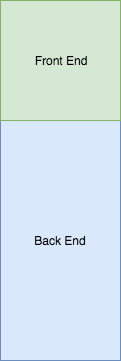
\includegraphics[height=5cm]{images/stack/abstract}
        \caption{The most abstract version of the site. This is separated into the front and back end. The back end code, represented in blue, runs on the server. The front end code, represented in green, runs on the tablet, phone, laptop or desktop that the user is operating.}
        \label{fig:abstract}
    \end{subfigure}
    ~
    \begin{subfigure}[b]{0.2\textwidth}
        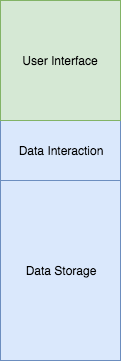
\includegraphics[height=5cm]{images/stack/abstract_medium}
        \caption{The abstract model with more concrete definitions of the location where the data is stored, the layer that serves as the interaction point between the two, and the interface.}
        \label{fig:abstract_medium}
    \end{subfigure}
    ~
    \begin{subfigure}[b]{0.2\textwidth}
        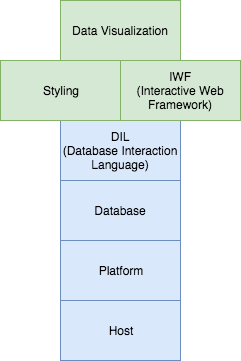
\includegraphics[height=5cm]{images/stack/general_tech}
        \caption{The same stack showing how each component breaks down into the technologies listed in the tech review. All sections on the middle right stack are summarized in the definitions section. }
        \label{fig:general_tech}
    \end{subfigure}
		~
    \begin{subfigure}[b]{0.2\textwidth}
        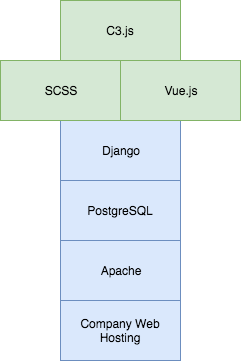
\includegraphics[height=5cm]{images/stack/chosen_tech}
        \caption{The full stack with the technologies BrewHops has selected for the project.}
        \label{fig:chosen_tech}
    \end{subfigure}
    \caption{The web tech stack with varying levels of specificity}\label{fig:animals}
		\end{figure}


	\subsection{Viewpoints}

		\subsubsection{Database Structure}

		The main purpose of our project is to bridge the gap between Brewers and the database at Ninkasi. Designing a functional database is key to making this project a success.
		Our database needs to connect the cellaring data on each beer for each day it is measured.
		The beers need to be connected to their predefined recipes.
		As brewers make decisions on what steps to complete next, the database needs to show what steps have already been completed via the information previously entered.
		It needs to keep track of who entered what data and whether the information entered is within the acceptable measurement ranges.

		The database system is based off of the excel spreadsheet currently in use by Ninkasi for storing data.
		Each beer is connected to a predefined recipe, and each beer currently in the cellar is associated with data collected each day, along with the alerts in place for that day.
		Our database design has 5 tables: TankActions, TankContents, TankInfo, BrandInfo, and Employees.
		Employees contains login usernames, passwords, and ID numbers for the employees.
		This is used for the login system and also for keeping track of who entered the TankContents information.
		The BrandInfo table keeps track of a brand’s recipe and the ranges associated with correct values.
		This is so that we can alert the brewers if temperature, gravity or pH are outside of the typical or safe levels.
		The last three tables are associated with the tanks, what’s inside of them, and the measurements of the beer in each tank.
		The TankInfo table contains TankID, beer name, batch number, generation, and volume to ferment.
		Each tank can have 1 or more TankContents, as each TankContent data set is taken on a different day and a batch can be in a tank for multiple weeks.
		TankContents contain the date on which the measurements took place, specific gravity, pH, ABV, temperature, and the EmployeeID who entered the data.
		TankActions hold actions that need to happen, the date, the TankID they are associated with, and the EmployeeID who satisfied the action, if they have fixed the problem.

		This system works for our project because it allows us to keep track of:

		\begin{itemize}
			\item What brand and batch are in each tank
			\item What is happening in that tank every day
			\item What actions need to be taken, and if they have been taken care of
			\item Who entered the data
			\item What the correct measurement ranges and ingredients are for each brand
		\end{itemize}

		\begin{itemize}
			\item Issues brought up:
			\item Inefficient query system if you want batch information over long periods of time
			\item BRITE is not anywhere in our diagram and the team is unsure where it belongs in the data structure
			\item Recipie is not a long varchar in the database
		\end{itemize}

		\subsubsection{RESTful API}

		Ninkasi needs all CRUD operations available to their user interfaces.
		To adhere with these standards, the API must be fully RESTful and expose the necessary GET, POST, PUT, PATCH, and DELETE routes.
		The API will have direct access into the database and will need to be secured per user so that only individuals with adequate permissions have access to certain API routing features.
		Other security concerns are that individuals outside of Ninkasi do not have access to the API.
		This will not be the BrewHops team’s primary concern as Ninkasi network security should handle these concerns when application is deployed.


		The user interfaces for the data management system need efficient access to all information stored in the database.
		The interfaces need to be able to get the data, insert new data, update old data, and delete incorrect data.
		Each route of the REST API will give access to these operations based on the type of operation performed on the url.

		Interfaces will need access to all information in the TankInfo table.
		To allow this, the routes on the /tanks url will handle retrieving all Tanks data, inserting and updating Tanks data, and retrieving batch information for each tank.

		What follows are each route and their purpose in the API:

		/api/tanks:
		\begin{itemize}
			\item GET: (queries TankInfo database table to get)
			\begin{itemize}
				\item TankID
				\item BrandID
				\item BATCH
				\item Yeast Generation
				\item Ferm\_To\_Vol
			\end{itemize}
			\item POST: (add a new Fermentation Tank to the database)
			\item /:id:
			\begin{itemize}
				\item GET: Query TankInfo for all batches produced in Tank
				\item POST: Add new batch to tank
				\item :id/:id\_batch: \\
					GET:
					\begin{itemize}
						\item Gets all rows of TankContent for BatchID
						\item PUT: update entire batch resource
						\item PATCH: update part of a batch resource
						\item DELETE: destroy a batch resource
					\end{itemize}
				\end{itemize}
		\end{itemize}


		The user interfaces also need access to the Employees table in the database to authenticate users and regulate permission capabilities of various users.
		To do this, we expose a /users route on the url that allows the interfaces to pull back information on all users or specific users.
		/api/users:
		\begin{itemize}
			\item GET: get a list of all users from Employee table
			\item POST: add user to Employee table

			\item /:id
			\begin{itemize}
				\item GET: get a user resource
				\item PUT: update entire user resource
				\item PATCH: update part of user resource
				\item DELETE: destroy user resource
			\end{itemize}
		\end{itemize}


		Our user interfaces may also need access to brand information on different beers.
		To facilitate these needs, we expose a /brand route on the url to access all brands or specific brands stored in the BrandInfo table.

		/api/brand:
		\begin{itemize}
			\item GET: retrieve list of all Ninkasi brands from BrandInfo
			\item POST: add a new brand

			\item /:id
			\begin{itemize}
				\item GET: retrieve all brand information
				\begin{itemize}
					\item Recipe
					\item List of batch ids currently in progress
				\end{itemize}
				\item PUT: update entire brand resource
				\item PATCH: partial update of brand resource
				\item DELETE: delete brand resource
			\end{itemize}
		\end{itemize}


		A RESTful API is important because it improves application maintainability and testability.
		Maintainability is a primary concern and requirement of this project.
		Ease of testing ensures the integrity of our final product and gives us further metrics to gage success.
		A REST API allows the BrewHops team to fully decouple\footnote{“decouple” means separate user interface concerns from server-side processing concerns} user interfaces from the backend processes.
		This is important because development on the user interface and the server-side support can work in parallel; the only dependency is how data is structured.
		Once data structure is determined for each route, our frontend developer can mock data\footnote{mocking data means to create a static data source for testing purposes} to test the interface while our backend developer builds out each route to the specifications.
		RESTful APIs also improve application testability by allowing developers to leverage testing frameworks designed for specific technologies.

		\subsubsection{General User Interface}

		The user interface needs to be designed in a way that is easily usable by the brewers.
		The UI design decisions will first be made by the BrewHops team.
		A prototype of the UI will be developed by the team based on the goals outlined by the client.
		The user interface will then go through an iterative feedback process where the client will provide changes, the team will revise the document and make new suggestions, which will then be returned to the client.
		This process will continue until both parties have verified that the design is both achievable by the development team and meets the goals of the client.
		Iterative design ensures that there is a balance of input, with multiple opportunities for everyone to contribute to the project.
		The BrewHops team has design experience, and it will be best for them to make a majority of the decisions about how the user interface will function.
		This will keep the burden of development off of the client, while still giving them an option to weigh in on changes they see being beneficial to their operations.

		\subsubsection{Mobile User Interface}

		The interface designed must be capable of running on both a large screen desktop and a mobile device.
		Basic data display and entry functionality must exist on mobile devices to meet project specifications.
		The process for designing the mobile interface will be the same iterative design process as the general interface.
		A mockup for mobile design shown in the appendix.
		This is the first form of the interface, and over the course of building the application, frequent feedback from the client will be taken into account to ensure that all goals are met in a way that works well for the client.
		Rationale for the mobile design is the same as that of the general user interface.

		\subsubsection{Maintainability}

		After we leave this project, Ninkasi needs other developers to be able to maintain our code and improve upon it.
		The most important thing is leaving good documentation in the project.
		This design document, along with the other papers written for the senior capstone course should serve as a good starting point.
		While the code is being written for the project, documentation on the code itself and its organizational structure should be used.
		Every folder with custom code in it should have a markdown document describing the contents of the documents.
		Assistance in locating code will come with use of common programming languages and design patterns.
		For example, ruby on rails is a popular web framework that comes with a base template.
		Common structures such as these are familiar to many programmers and should keep the project from being too difficult to interpret for new developers.
		Open source projects have been struggling with ensuing that contributors know how to read the code that exists in the project, and write changes that are useful to the project.
		There has been a development of general design strategies used in the open source community to ensure a maintainable project, and utilizing these strategies will create a project that will be maintainable for whoever works on the project after the BrewHops team is done.


		\section{Appendix}
		\subsection{Mobile Design}
		\centering
		\begin{tabular}{ll}
				Home & Menu \\
				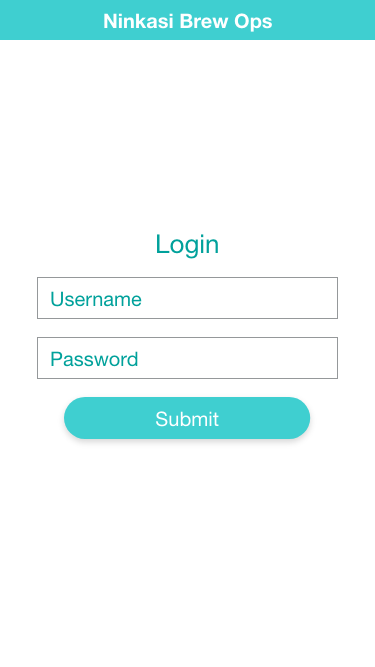
\includegraphics[scale=.3]{images/mobile/home} & 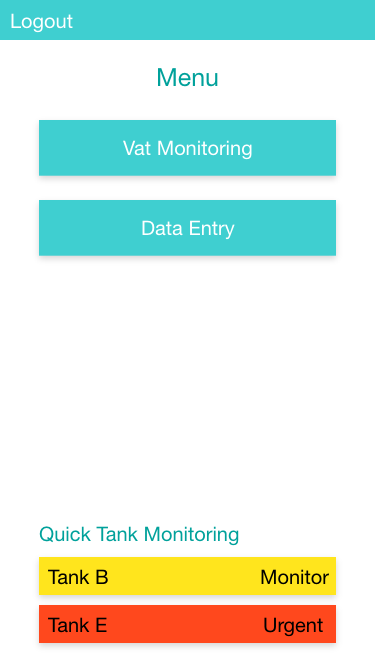
\includegraphics[scale=.3]{images/mobile/menu} \\
				Data Entry & Confirmation Page \\
				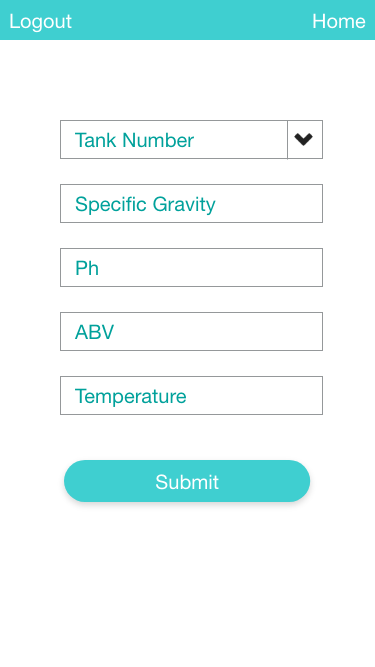
\includegraphics[scale=.3]{images/mobile/data_entry} & 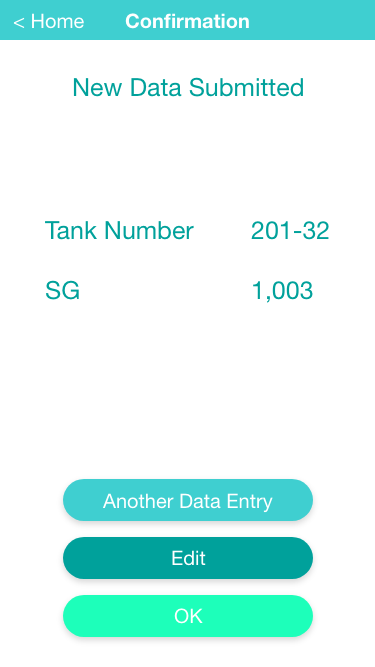
\includegraphics[scale=.3]{images/mobile/confirmation_page} \\
				Tank Monitoring & Tank Info \\
				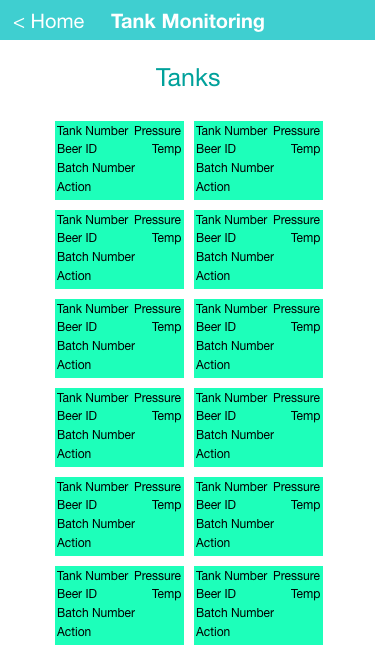
\includegraphics[scale=.3]{images/mobile/tank_monitoring} & 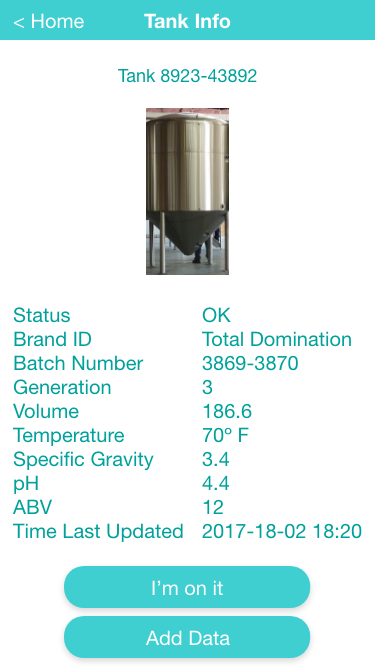
\includegraphics[scale=.3]{images/mobile/tank_info} \\
		\end{tabular}

		\subsection{Desktop Design}
		\begin{tabular}{l}
				Admin \\
				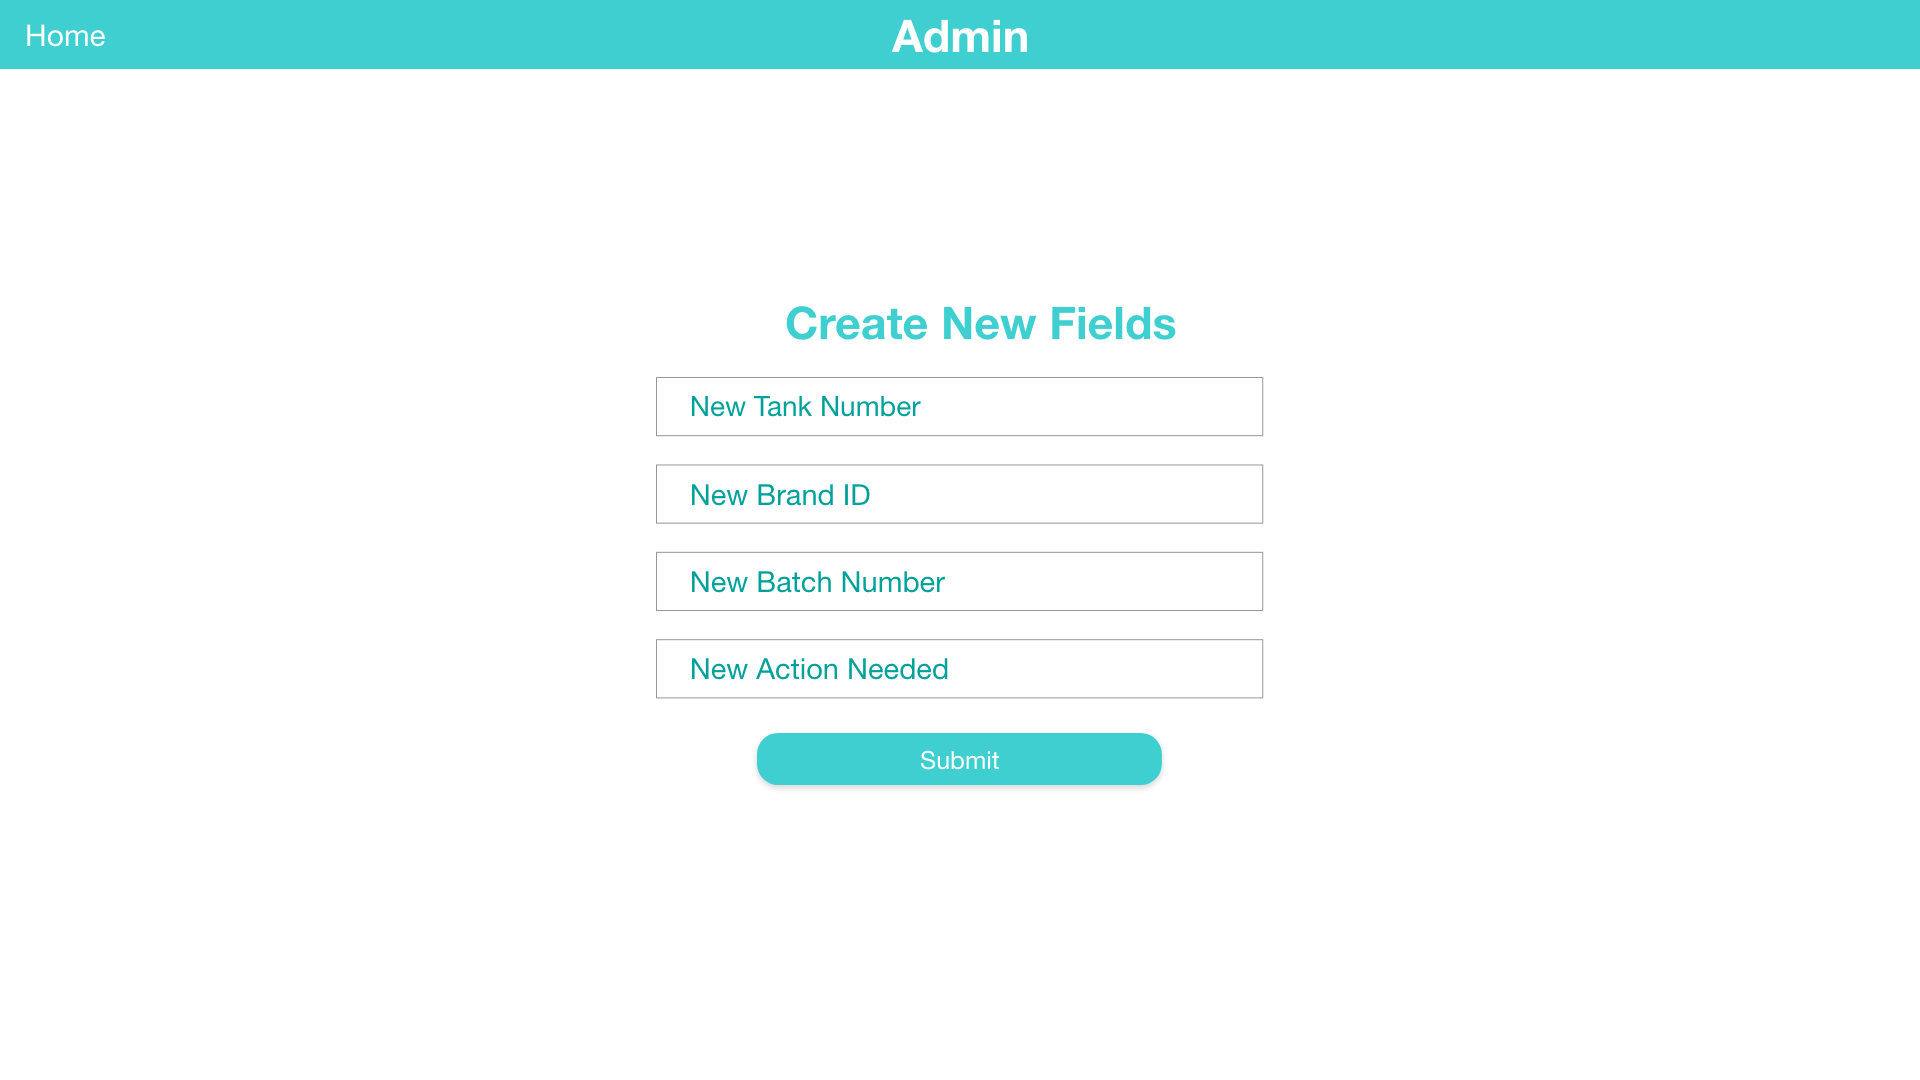
\includegraphics[scale=.15]{images/web/admin} \\
				Home \\
				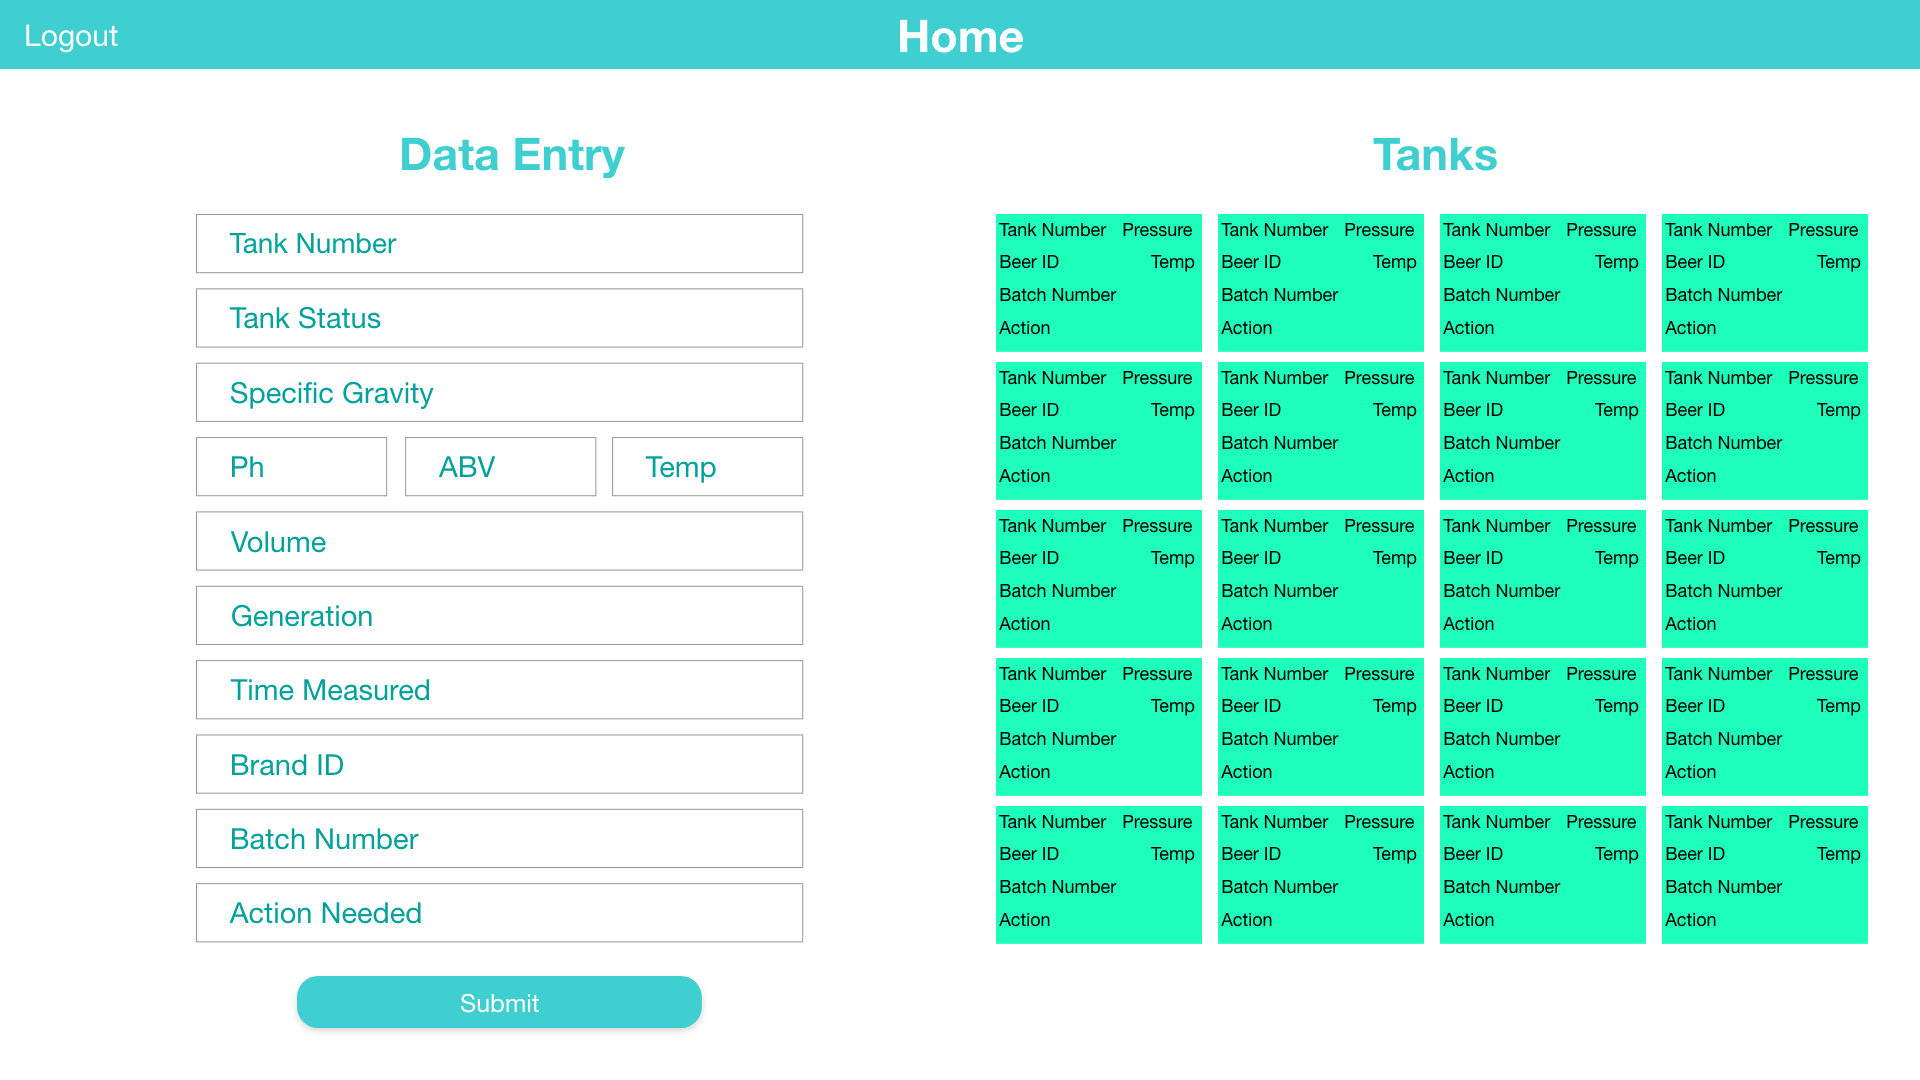
\includegraphics[scale=.15]{images/web/home} \\
				Login \\
				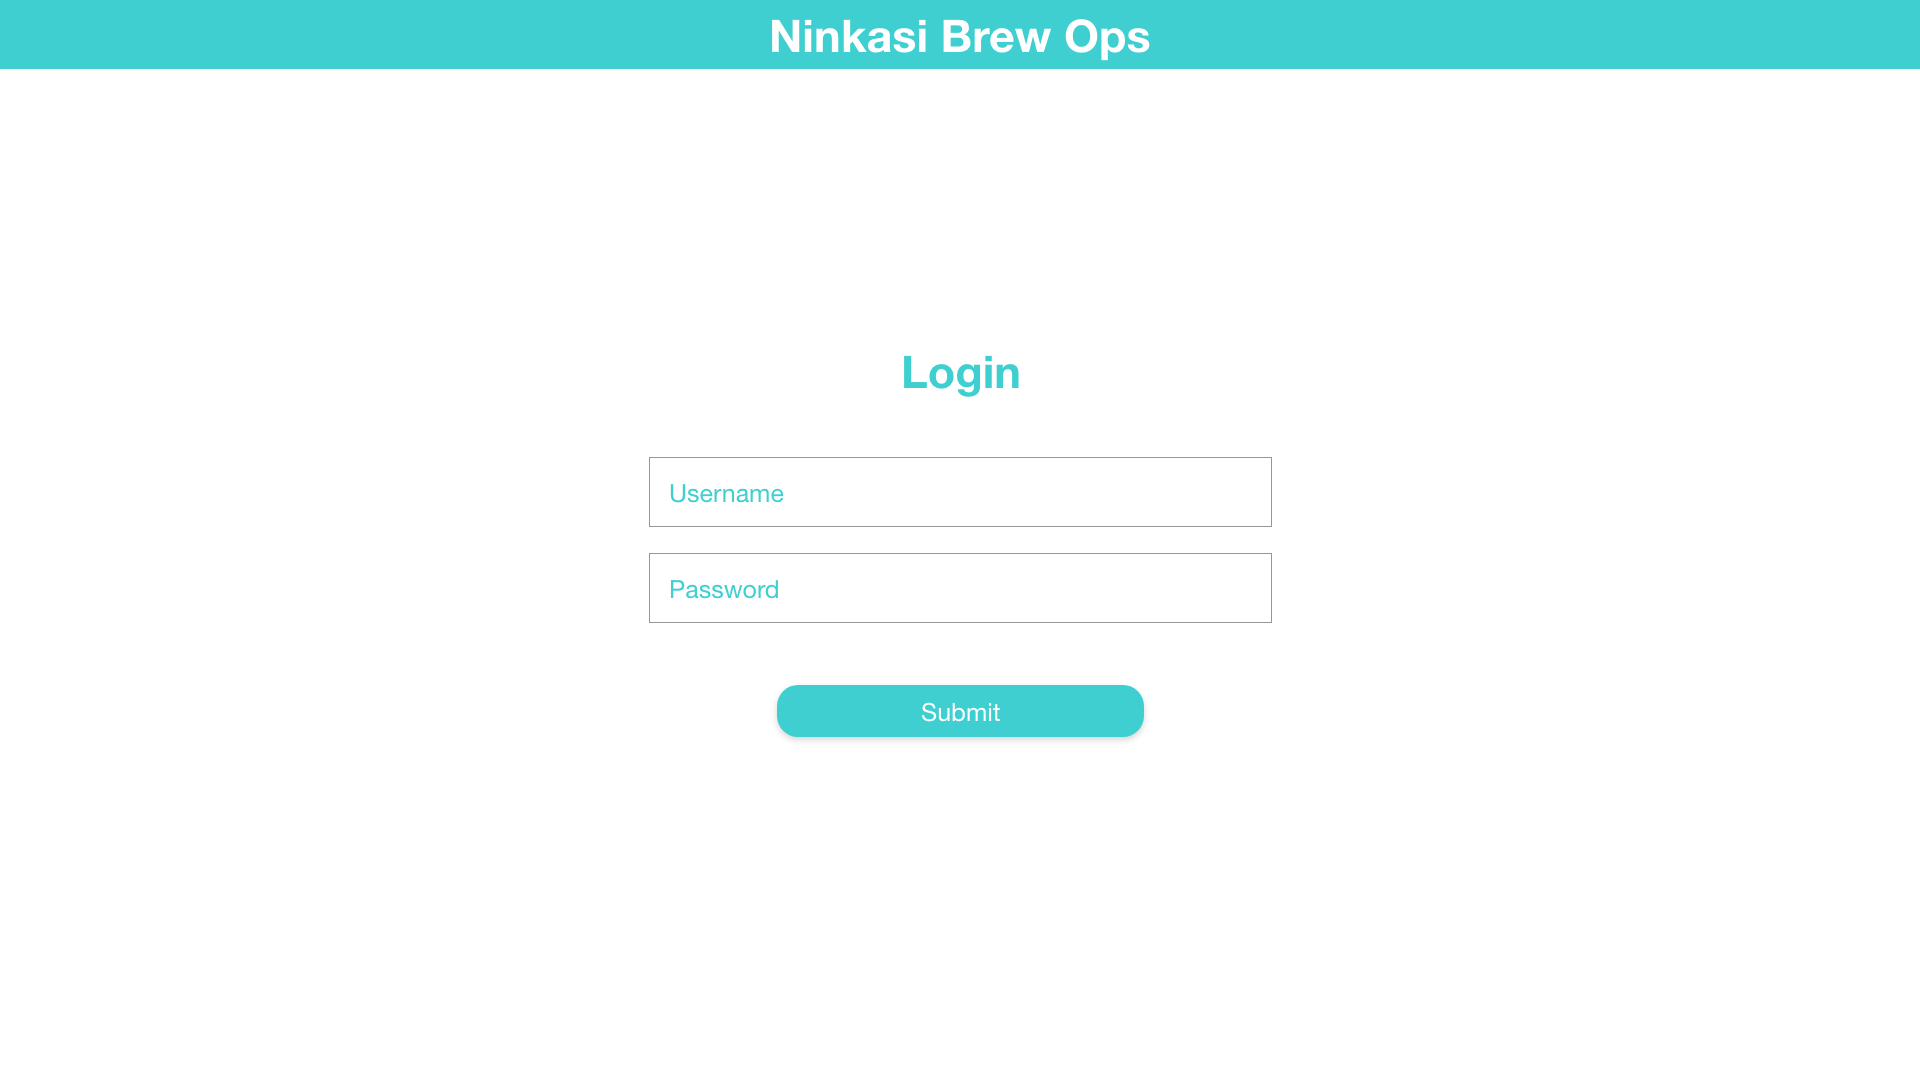
\includegraphics[scale=.15]{images/web/login} \\
				Tank Info \\
				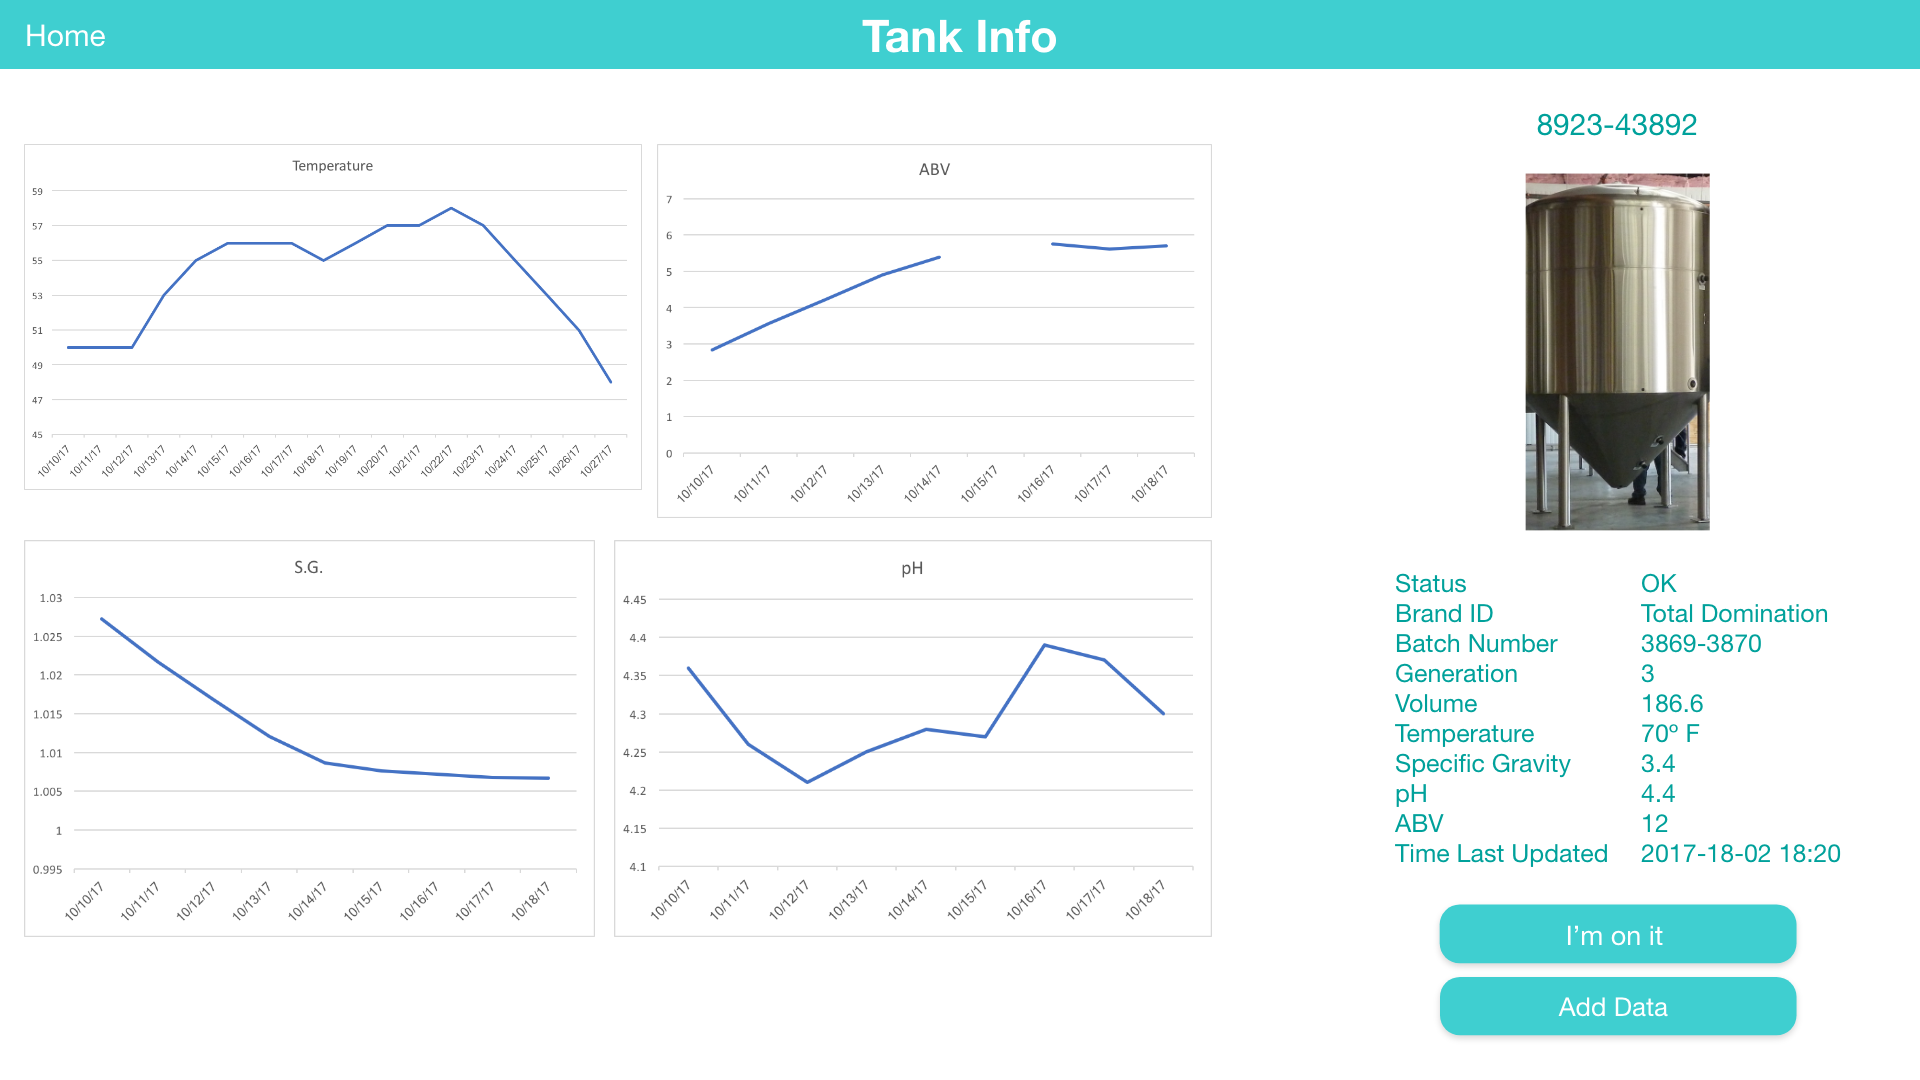
\includegraphics[scale=.15]{images/web/tank_info} \\
		\end{tabular}

\end{document}
